\chapter{Estudo de simulação}

%=====================================================

Com o objetivo de avaliar o poder do teste Wald em testes de hipóteses sobre parâmetros de McGLMs, foram executados estudos de simulação. Nestas simulações avaliamos o comportamento da proposta para três distribuições de probabilidade: Normal, Poisson e Bernoulli. Simulamos cenários univariados e também trivariados com diferentes tamanhos amostrais para verificar as propriedades dos testes sobre parâmetros de regressão, dispersão e potência.

Para simular conjuntos de dados univariados foram usadas bibliotecas padrões do R. Para simular conjuntos de dados com múltiplas respostas seguindo distribuição Normal, foi usada a biblioteca R \emph{mvtnorm} \citep{mvtnorm1}, \citep{mvtnorm2}. Para as outras distribuições foi utilizado o método NORTA \citep{cario1997modeling} implementado na biblioteca R \emph{NORTARA} \citep{nortara}.

\section{Parâmetros de regressão}

Para avaliação de hipóteses sobre parâmetros de regressão foram considerados tamanhos amostrais de 50, 100, 250, 500 e 1000. Foram gerados 500 conjuntos de dados para cada tamanho amostral simulando uma situação com uma variável explicativa categórica de 4 níveis. Para distribuição Normal os parâmetros de regressão usados foram: $\beta_0 = 5$, $\beta_1 = 0$, $\beta_2 = 0$, $\beta_3 = 0$. Para a distribuição Poisson os parâmetros de regressão usados foram: $\beta_0 = 2,3$, $\beta_1 = 0$, $\beta_2 = 0$, $\beta_3 = 0$. E para a distribuição Bernoulli os parâmetros de regressão usados foram: $\beta_0 = 0,5$, $\beta_1 = 0$, $\beta_2 = 0$, $\beta_3 = 0$. Os valores foram escolhidos de tal modo que o coeficiente de variação para distribuição Normal fosse de 20\%, as contagens para Poisson fossem próximas de 10 e a probabilidade de sucesso da Bernoulli fosse aproximadamente 0,6. Foram avaliados cenários univariados e trivariados com estas características. Para os cenários trivariados, existem 4 parâmetros por resposta que seguem as configurações descritas. Para cada amostra gerada foi ajustado um McGLM. As funções de ligação e variância para cada distribuição são apresentadas na \autoref{tab:link_var}. 

\begin{table}[H]
\centering
\begin{tabular}{ccc}
\hline
Distribuição & Função de ligação & Função de variância \\ \hline
Normal       & Identidade        & Constante           \\
Poisson      & Logarítmica       & Tweedie             \\
Bernoulli    & Logito            & Binomial            \\ \hline
\end{tabular}
\caption{Funções de ligação e variância utilizadas nos modelos para cada distribuição simulada.}
\label{tab:link_var}
\end{table}

Em todos os casos o preditor matricial para a matriz de variância e covariância foi especificado de forma a explicitar que as observações são independentes dentro de cada resposta. A correlação entre respostas no caso trivariado é dada pela matriz $\Sigma_b$ descrita na \autoref{eq:correlacao}.

\begin{equation} \label{eq:correlacao}
\Sigma_b = 
\begin{bmatrix}
1    & 0,75 & 0,5  \\
0,75 & 1    & 0,25 \\
0,5  & 0,25 & 1    \\
\end{bmatrix}
\end{equation}

Com os modelos ajustados, o procedimento consistiu em variar as hipóteses testadas sobre os parâmetros simulados. Consideramos 20 diferentes hipóteses baseadas em um decréscimo de $\beta_0/20$ e distribuição deste decréscimo nos demais $\beta$s da hipótese nula. Para cada ponto avaliamos o percentual de rejeição da hipótese nula. A ideia é verificar o que ocorre quando afastamos as hipóteses nulas dos reais valores dos parâmetros. Espera-se que no primeiro ponto haja um percentual de rejeição baixo, pois a hipótese nula corresponde aos reais valores dos parâmetros. Para os demais pontos espera-se que o percentual de rejeição aumente gradativamente, pois as hipóteses afastam-se dos valores originalmente simulados. As hipóteses testadas para as respostas com distribuição Normal são mostradas na \autoref{tab:th_normal}; as hipóteses testadas para respostas seguindo distribuição Poisson estão na \autoref{tab:th_poisson} e as hipóteses para as respostas Bernoullis são mostradas na \autoref{tab:th_bernoulli}.

\begin{table}[H]
\centering
\begin{tabular}{ccccc}
\hline
          & $\beta_0$ & $\beta_1$ & $\beta_2$ & $\beta_3$ \\ \hline
$H_{01}$  & 5         & 0         & 0         & 0         \\
$H_{02}$  & 4,75      & 0,083     & 0,083     & 0,083     \\
$H_{03}$  & 4,5       & 0,166     & 0,166     & 0,166     \\
$H_{04}$  & 4,25      & 0,25      & 0,25      & 0,25      \\
$H_{05}$  & 4         & 0,333     & 0,333     & 0,333     \\
$H_{06}$  & 3,75      & 0,416     & 0,416     & 0,416     \\
$H_{07}$  & 3,5       & 0,5       & 0,5       & 0,5       \\
$H_{08}$  & 3,25      & 0,583     & 0,583     & 0,583     \\
$H_{09}$  & 3         & 0,666     & 0,666     & 0,666     \\
$H_{010}$ & 2,75      & 0,75      & 0,75      & 0,75      \\
$H_{011}$ & 2,5       & 0,833     & 0,833     & 0,833     \\
$H_{012}$ & 2,25      & 0,916     & 0,916     & 0,916     \\
$H_{013}$ & 2         & 1         & 1         & 1         \\
$H_{014}$ & 1,75      & 1,083     & 1,083     & 1,083     \\
$H_{015}$ & 1,5       & 1,166     & 1,166     & 1,166     \\
$H_{016}$ & 1,25      & 1,25      & 1,25      & 1,25      \\
$H_{017}$ & 1         & 1,33      & 1,33      & 1,33      \\
$H_{018}$ & 0,75      & 1,41      & 1,41      & 1,41      \\
$H_{019}$ & 0,5       & 1,5       & 1,5       & 1,5       \\
$H_{020}$ & 0,25      & 1,58      & 1,58      & 1,58      \\ \hline
\end{tabular}
\caption{Hipóteses testadas para distribuição Normal.}
\label{tab:th_normal}
\end{table}

\begin{table}[H]
\centering
\begin{tabular}{ccccc}
\hline
          & $\beta_0$ & $\beta_1$ & $\beta_2$ & $\beta_3$ \\ \hline
$H_{01}$  & 2,3       & 0         & 0         & 0         \\
$H_{02}$  & 2,185     & 0,0383    & 0,0383    & 0,0383    \\
$H_{03}$  & 2,07      & 0,0766    & 0,0766    & 0,0766    \\
$H_{04}$  & 1,955     & 0,115     & 0,115     & 0,115     \\
$H_{05}$  & 1,84      & 0,153     & 0,153     & 0,153     \\
$H_{06}$  & 1,725     & 0,192     & 0,191     & 0,191     \\
$H_{07}$  & 1,61      & 0,23      & 0,23      & 0,23      \\
$H_{08}$  & 1,495     & 0,268     & 0,268     & 0,268     \\
$H_{09}$  & 1,38      & 0,306     & 0,306     & 0,306     \\
$H_{010}$ & 1,265     & 0,345     & 0,345     & 0,345     \\
$H_{011}$ & 1,15      & 0,383     & 0,383     & 0,383     \\
$H_{012}$ & 1,035     & 0,421     & 0,421     & 0,421     \\
$H_{013}$ & 0,92      & 0,46      & 0,46      & 0,46      \\
$H_{014}$ & 0,805     & 0,498     & 0,498     & 0,498     \\
$H_{015}$ & 0,69      & 0,536     & 0,536     & 0,536     \\
$H_{016}$ & 0,575     & 0,575     & 0,575     & 0,575     \\
$H_{017}$ & 0,46      & 0,613     & 0,613     & 0,613     \\
$H_{018}$ & 0,345     & 0,651     & 0,651     & 0,651     \\
$H_{019}$ & 0,23      & 0,69      & 0,69      & 0,69      \\
$H_{020}$ & 0,115     & 0,728     & 0,728     & 0,728     \\ \hline
\end{tabular}
\caption{Hipóteses testadas para distribuição Poisson.}
\label{tab:th_poisson}
\end{table}


\begin{table}[H]
\centering
\begin{tabular}{ccccc}
\hline
          & $\beta_0$ & $\beta_1$ & $\beta_2$ & $\beta_3$ \\ \hline
$H_{01}$  & 0,5       & 0         & 0         & 0         \\
$H_{02}$  & 0,475     & 0,008     & 0,008     & 0,008     \\
$H_{03}$  & 0,45      & 0,016     & 0,016     & 0,016     \\
$H_{04}$  & 0,425     & 0,025     & 0,025     & 0,025     \\
$H_{05}$  & 0,4       & 0,033     & 0,033     & 0,033     \\
$H_{06}$  & 0,375     & 0,041     & 0,041     & 0,041     \\
$H_{07}$  & 0,35      & 0,05      & 0,05      & 0,05      \\
$H_{08}$  & 0,325     & 0,058     & 0,058     & 0,058     \\
$H_{09}$  & 0,3       & 0,066     & 0,066     & 0,066     \\
$H_{010}$ & 0,275     & 0,075     & 0,075     & 0,075     \\
$H_{011}$ & 0,25      & 0,083     & 0,083     & 0,083     \\
$H_{012}$ & 0,225     & 0,091     & 0,091     & 0,091     \\
$H_{013}$ & 0,2       & 0,1       & 0,1       & 0,1       \\
$H_{014}$ & 0,175     & 0,108     & 0,108     & 0,108     \\
$H_{015}$ & 0,15      & 0,116     & 0,116     & 0,116     \\
$H_{016}$ & 0,125     & 0,125     & 0,125     & 0,125     \\
$H_{017}$ & 0,099     & 0,133     & 0,133     & 0,133     \\
$H_{018}$ & 0,074     & 0,141     & 0,141     & 0,141     \\
$H_{019}$ & 0,049     & 0,15      & 0,15      & 0,15      \\
$H_{020}$ & 0,024     & 0,158     & 0,158     & 0,158     \\ \hline
\end{tabular}
\caption{Hipóteses testadas para distribuição Bernoulli.}
\label{tab:th_bernoulli}
\end{table}

Para representar graficamente os resultados tomamos a distância euclideana de cada vetor de hipóteses com relação ao vetor usado para simular os dados. Adicionalmente dividimos o vetor de distâncias pelo seu desvio padrão para obter distâncias em uma mesma escala, independente dos parâmetros de regressão. Os resultados são apresentados na \autoref{fig:betas}.

\begin{figure}[H]
\centering
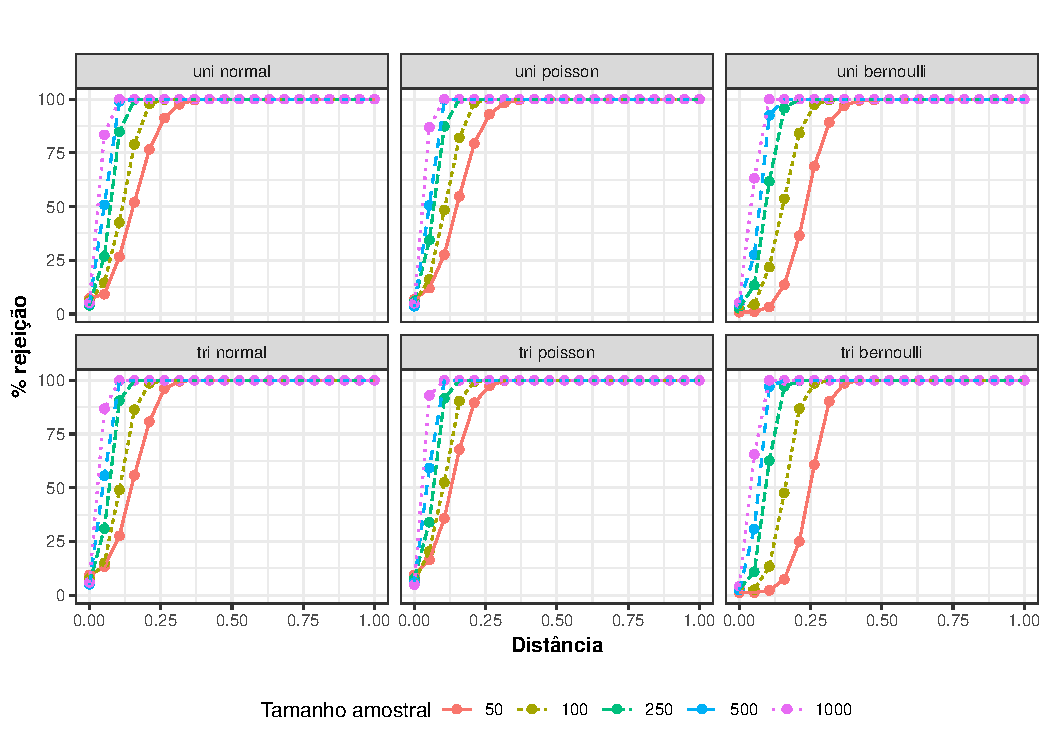
\includegraphics[width=15cm]{/home/lacf14/msc/4_dissertacao/6-simulacao/betas.pdf}
\caption{Resultados do estudo de simulação para os parâmetros de regressão.}
\label{fig:betas}
\end{figure}

De modo geral, quanto mais distante a hipótese é dos valores inicialmente simulados, maior é o percentual de rejeição. Como esperado, os menores percentuais foram observados na hipótese igual aos valores simulados. Tanto para cenários univariados e trivariados com distribuição Normal e Poisson, o percentual de rejeição foi próximo a 10\% quando a hipótese era igual aos valores simulados mesmo com tamanhos amostrais reduzidos, como 50 e 100. Conforme afastamos a hipótese dos valores simulados o percentual de rejeição aumentou mesmo com hipóteses pouco diferentes dos valores simulados. Também como esperado há um desempenho inferior para distribuição bernoulli no caso univariado e trivariado de forma que há indício de que para funcionamento correto do teste há necessidade de tamanhos amostrais maiores.

\section{Parâmetros de dispersão}

Para avaliação de hipóteses sobre parâmetros de dispersão foram considerados os mesmos tamanhos amostrais: 50, 100, 250, 500 e 1000. Contudo, os conjuntos de dados simulam uma situação em que cada unidade amostral fornece 5 medidas ao conjunto de dados. Foram gerados 500 conjuntos de dados para cada tamanho amostral e distribuição. Para distribuição Normal foram simulados vetores com média 5 e desvio padrão igual a 1. Para distribuição Poisson foram simuladas contagens com taxa igual a 10. Para distribuição Bernoulli foram simulados vetores de uma variável dicotômica com probabilidade de sucesso igual a 0,6.

Em todos os casos, os parâmetros de dispersão para gerar os conjuntos de dados foram fixados em 0,5 e não foi incluído efeito de variáveis explicativas. Foram avaliados cenários univariados e trivariados com estas características. Para cada amostra gerada foi ajustado um McGLM com funções de ligação e variância tal como descrito na \autoref{tab:link_var}. Nos cenários trivariados a correlação entre respostas é dada pela \autoref{eq:correlacao}.

Neste caso, como as medidas são correlacionadas dentro de cada resposta, é necessário especificar um preditor matricial que deixa explícito que as medidas são correlacionadas. O objetivo é testar hipóteses sobre os parâmetros de dispersão associados a este preditor matricial. 

Com os modelos ajustados, o procedimento consistiu em variar as hipóteses testadas sobre os parâmetros simulados. Consideramos 20 diferentes hipóteses baseadas em um decréscimo sucessivo de $0,5/20$ para cada hipótese nula testeda. Para cada ponto avaliamos o percentual de rejeição da hipótese nula. A ideia é afastar sucessivamente a hipótese dos valores simulados e avaliar se conforme afastamos a hipótese dos valores verdadeiros, o percentual de rejeição aumenta. As hipóteses testadas são mostradas na \autoref{tab:th_taus}.

\begin{table}[H]
\centering
\begin{tabular}{ccc}
\hline
          & $\tau_0$ & $\tau_1$ \\ \hline
$H_{01}$  & 0,5      & 0,5      \\
$H_{02}$  & 0,475    & 0,475    \\
$H_{03}$  & 0,45     & 0,45     \\
$H_{04}$  & 0,425    & 0,425    \\
$H_{05}$  & 0,4      & 0,4      \\
$H_{06}$  & 0,375    & 0,375    \\
$H_{07}$  & 0,35     & 0,35     \\
$H_{08}$  & 0,325    & 0,325    \\
$H_{09}$  & 0,3      & 0,3      \\
$H_{010}$ & 0,275    & 0,275    \\
$H_{011}$ & 0,25     & 0,25     \\
$H_{012}$ & 0,225    & 0,225    \\
$H_{013}$ & 0,2      & 0,2      \\
$H_{014}$ & 0,175    & 0,175    \\
$H_{015}$ & 0,15     & 0,15     \\
$H_{016}$ & 0,125    & 0,125    \\
$H_{017}$ & 0,099    & 0,099    \\
$H_{018}$ & 0,074    & 0,074    \\
$H_{019}$ & 0,049    & 0,049    \\
$H_{020}$ & 0,024    & 0,024    \\ \hline
\end{tabular}
\caption{Hipóteses testadas para parâmetros de dispersão.}
\label{tab:th_taus}
\end{table}

Do mesmo modo que foi feito para os parâmetros de regressão, foi tomada a distância euclideana de cada vetor de hipóteses com relação ao vetor usado para simular os dados; e o vetor de distâncias foi padronizado para obter distâncias em uma mesma escala, independente dos parâmetros simulados. Os resultados são apresentados na \autoref{fig:taus}.

\begin{figure}[H]
\centering
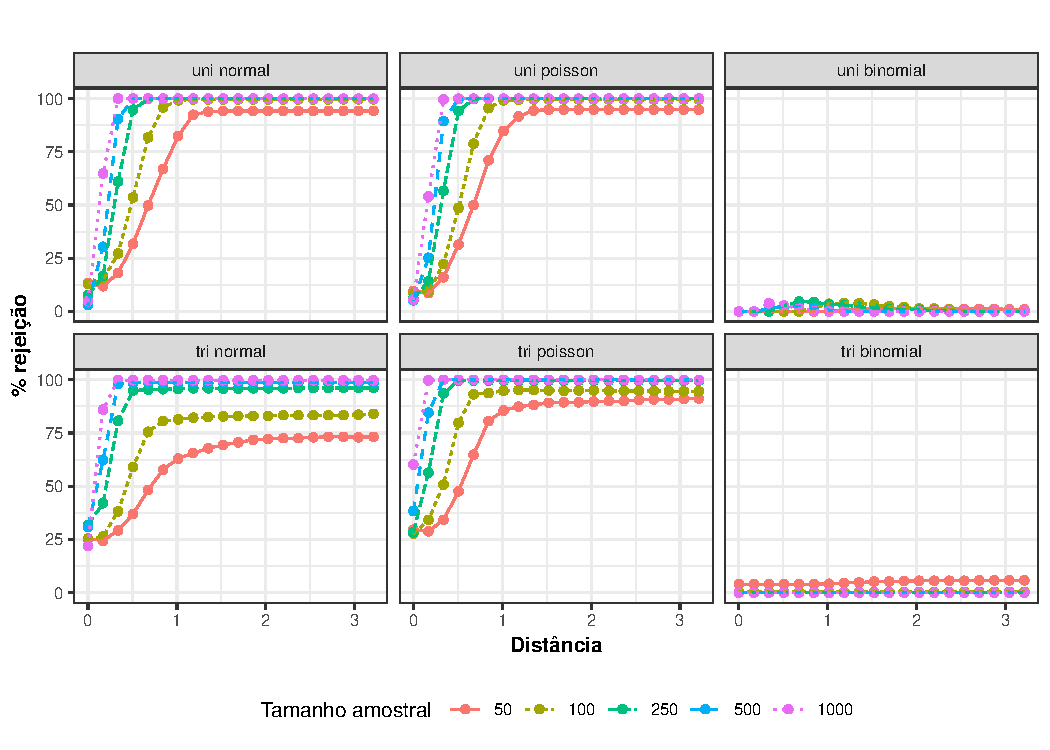
\includegraphics[width=15cm]{/home/lacf14/msc/4_dissertacao/6-simulacao/taus.pdf}
\caption{Resultados do estudo de simulação para os parâmetros de dispersão.}
\label{fig:taus}
\end{figure}

Assim como observado para os parâmetros de regressão, o comportamento dos gráficos mostra que, para distribuição Normal e Poisson, quanto mais distante a hipótese é dos valores inicialmente simulados, maior é o percentual de rejeição, e os menores percentuais são observados em hipóteses próximas aos valores simulados. 

Para os cenários univariados o comportamento dos testes se mostrou satisfatório com tamanhos amostrais maiores que 100 pois na primeira hipótese testada o percentual de rejeição se mostrou menor que 10\%.

Contudo o percentual de rejeição para hipóteses iguais aos valores simulados é considerávelmente distante do esperado para os cenários trivariados, nestes casos observamos percentuais de rejeição maiores que 20\%, apesar de que quanto mais distante dos valores simulados maior é o percentual de rejeição. Já para distribuição Bernoulli não foram obtidos resultados satisfatórios.

\section{Parâmetros de potência}

Para avaliação de hipóteses sobre parâmetros de potência foram novamente considerados tamanhos amostrais de 50, 100, 250, 500 e 1000. Foram gerados 500 conjuntos de dados para cada tamanho amostral simulando uma situação com uma variável explicativa categórica de 2 níveis. Para distribuição Normal os parâmetros de regressão usados foram: $\beta_0 = 3$ e $\beta_1 = 2$. Para a distribuição Poisson os parâmetros de regressão usados foram: $\beta_0 = 1,3$ e $\beta_1 = 0,7$. E para a distribuição Bernoulli os parâmetros de regressão usados foram: $\beta_0 = 0,35$ e $\beta_1 = 0,15$. Os valores foram escolhidos de tal modo que haja um parâmetro de regressão com efeito significativo para que seja possível estimar os parâmetros de potência. Foram avaliados cenários univariados e trivariados com estas características.

A correlação entre respostas no caso trivariado é dada pela matriz $\Sigma_b$ descrita na \autoref{eq:correlacao}. Para cada amostra gerada foi ajustado um McGLM em que para todos os casos o preditor matricial foi especificado de forma a explicitar que as observações são independentes dentro de cada resposta.

Similar ao que foi feito para parâmetros de regressão e dispersão, o procedimento consistiu em variar as hipóteses testadas sobre os parâmetros simulados. Nestas configurações, espera-se que o parâmetro de potência seja 0, 1 e 1 para as distribuições Normal, Poisson e Bernoulli, respectivamente. Para avaliar o teste, consideramos 20 diferentes hipóteses baseadas em um acréscimo sucessivo de $2/20$ para cada hipótese nula testeda. Para cada ponto avaliamos o percentual de rejeição da hipótese nula. Tal como nos casos anteriores espera-se que, afastando os valores da hipótese dos valores verdadeiros, o número de rejeições cresça. As hipóteses testadas são mostradas na \autoref{tab:th_p}.

\begin{table}[H]
\centering
\begin{tabular}{cccc}
\hline
          & Normal & Poisson & Bernoulli \\ \hline
$H_{01}$  & 0      & 1       & 1         \\
$H_{02}$  & 0,1    & 1,1     & 1,1       \\
$H_{03}$  & 0,2    & 1,2     & 1,2       \\
$H_{04}$  & 0,3    & 1,3     & 1,3       \\
$H_{05}$  & 0,4    & 1,4     & 1,4       \\
$H_{06}$  & 0,5    & 1,5     & 1,5       \\
$H_{07}$  & 0,6    & 1,6     & 1,6       \\
$H_{08}$  & 0,7    & 1,7     & 1,7       \\
$H_{09}$  & 0,8    & 1,8     & 1,8       \\
$H_{010}$ & 0,9    & 1,9     & 1,9       \\
$H_{011}$ & 1      & 2       & 2         \\
$H_{012}$ & 1,1    & 2,1     & 2,1       \\
$H_{013}$ & 1,2    & 2,2     & 2,2       \\
$H_{014}$ & 1,3    & 2,3     & 2,3       \\
$H_{015}$ & 1,4    & 2,4     & 2,4       \\
$H_{016}$ & 1,5    & 2,5     & 2,5       \\
$H_{017}$ & 1,6    & 2,6     & 2,6       \\
$H_{018}$ & 1,7    & 2,7     & 2,7       \\
$H_{019}$ & 1,8    & 2,8     & 2,8       \\
$H_{020}$ & 1,9    & 2,9     & 2,9       \\ \hline
\end{tabular}
\caption{Hipóteses testadas para parâmetros de potência para cada distribuição simulada.}
\label{tab:th_p}
\end{table}


Da mesma forma que o realizado para o estudo sobre parâmetros de regressão e dispersão, tomamos a distância euclideana de cada vetor de hipóteses com relação ao vetor usado para simular os dados e padronizamos o vetor. Os resultados são apresentados na \autoref{fig:ps}.

\begin{figure}[H]
\centering
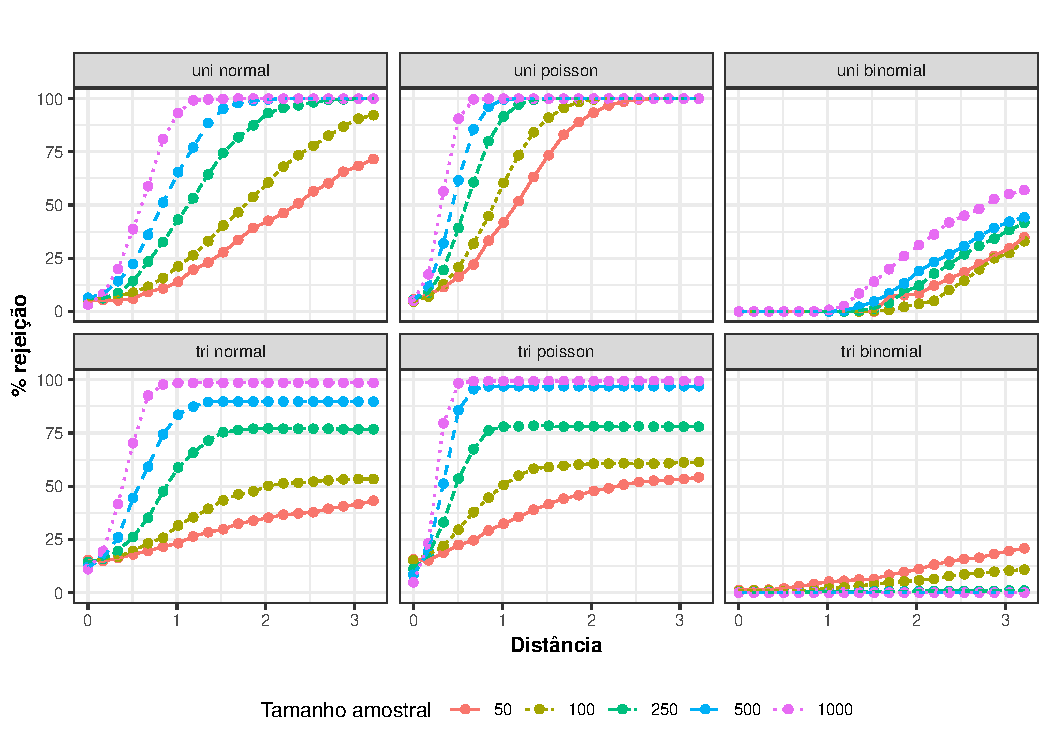
\includegraphics[width=15cm]{/home/lacf14/msc/4_dissertacao/6-simulacao/ps.pdf}
\caption{Resultados do estudo de simulação para os parâmetros de potência.}
\label{fig:ps}
\end{figure}

Os resultados para os parâmetros de potência nos casos univariados com distribuição Normal e Poisson se mostraram bastante satisfatórios, com percentuais de rejeição próximos a 5\% na hipótese igual aos valores simulados com percentual de rejeição crescente nas hipóteses mais afastadas. Tal como ocorreu para os parâmetros de regressão há um desempenho inferior para distribuição Bernoulli no caso univariado indicando que existe a necessidade de tamanhos amostrais maiores para realização dos testes.

Para os cenários trivariados com distribuição Normal e Poisson, o percentual de rejeição cresce a medida que afastamos as hipóteses dos valores simulados, contudo o percentual de rejeição na hipótese igual aos valores simulados é próximo de 15\%. Já para distribuição Bernoulli no cenário trivariado não foram obtidos resultados satisfatórios.

%=====================================================

\textbf{TODO}

\begin{itemize}

  \item \textbf{VERIFICAR COM O WAGNER COMO COLOCAR OS GRÁFICOS}

  \item \textbf{ATUALIZAR FACET BINOMIAL -> BERNOULLI}

  \item \textbf{MANTER TABELAS COM AS HIPÓTESES TESTADAS?}

\end{itemize}

%=====================================================